
\documentclass[letterpaper,hide notes,xcolor={table,svgnames},pdftex,10pt]{beamer}
\def\showexamples{t}


%\usepackage[svgnames]{xcolor}

%% Demo talk
%\documentclass[letterpaper,notes=show]{beamer}

\usecolortheme{crane}
\setbeamertemplate{navigation symbols}{}

\usetheme{MyPittsburgh}
%\usetheme{Frankfurt}

%\usepackage{tipa}

\usepackage{hyperref}
\usepackage{graphicx,xspace}
\usepackage[normalem]{ulem}
\usepackage{multicol}
\usepackage{amsmath,amssymb,amsthm,graphicx,xspace}
\newcommand\SF[1]{$\bigstar$\footnote{SF: #1}}

\usepackage[default]{sourcesanspro}
\usepackage[T1]{fontenc}

\newcounter{tmpnumSlide}
\newcounter{tmpnumNote}

% old question code
%\newcommand\question[1]{{$\bigstar$ \small \onlySlide{2}{#1}}}
% \newcommand\nquestion[1]{\ifdefined \presentationonly \textcircled{?} \fi \note{\par{\Large \textbf{?}} #1}}
% \newcommand\nanswer[1]{\note{\par{\Large \textbf{A}} #1}}


 \newcommand\mnote[1]{%
   \addtocounter{tmpnumSlide}{1}
   \ifdefined\showcues {~\tiny\fbox{\arabic{tmpnumSlide}}}\fi
   \note{\setlength{\parskip}{1ex}\addtocounter{tmpnumNote}{1}\textbf{\Large \arabic{tmpnumNote}:} {#1\par}}}

\newcommand\mmnote[1]{\note{\setlength{\parskip}{1ex}#1\par}}

%\newcommand\mnote[2][]{\ifdefined\handoutwithnotes {~\tiny\fbox{#1}}\fi
% \note{\setlength{\parskip}{1ex}\textbf{\Large #1:} #2\par}}

%\newcommand\mnote[2][]{{\tiny\fbox{#1}} \note{\setlength{\parskip}{1ex}\textbf{\Large #1:} #2\par}}

\newcommand\mquestion[2]{{~\color{red}\fbox{?}}\note{\setlength{\parskip}{1ex}\par{\Large \textbf{?}} #1} \note{\setlength{\parskip}{1ex}\par{\Large \textbf{A}} #2\par}\ifdefined \presentationonly \pause \fi}

\newcommand\blackboard[1]{%
\ifdefined   \showblackboard
  {#1}
  \else {\begin{center} \fbox{\colorbox{blue!30}{%
         \begin{minipage}{.95\linewidth}%
           \hspace{\stretch{1}} Some space intentionally left blank; done at the blackboard.%
         \end{minipage}}}\end{center}}%
         \fi%
}



%\newcommand\q{\tikz \node[thick,color=black,shape=circle]{?};}
%\newcommand\q{\ifdefined \presentationonly \textcircled{?} \fi}

\usepackage{listings}
\lstset{%
  keywordstyle=\bfseries,
  aboveskip=15pt,
  belowskip=15pt,
  captionpos=b,
  identifierstyle=\ttfamily,
  escapeinside={(*@}{@*)},
  stringstyle=\ttfamiliy,
  frame=lines,
  numbers=left, basicstyle=\scriptsize, numberstyle=\tiny, stepnumber=0, numbersep=2pt}

\usepackage{siunitx}
\newcommand\sius[1]{\num[group-separator = {,}]{#1}\si{\micro\second}}
\newcommand\sims[1]{\num[group-separator = {,}]{#1}\si{\milli\second}}
\newcommand\sins[1]{\num[group-separator = {,}]{#1}\si{\nano\second}}
\sisetup{group-separator = {,}, group-digits = true}

%% -------------------- tikz --------------------
\usepackage{tikz}
\usetikzlibrary{positioning}
\usetikzlibrary{arrows,backgrounds,automata,decorations.shapes,decorations.pathmorphing,decorations.markings,decorations.text}

\tikzstyle{place}=[circle,draw=blue!50,fill=blue!20,thick, inner sep=0pt,minimum size=6mm]
\tikzstyle{transition}=[rectangle,draw=black!50,fill=black!20,thick, inner sep=0pt,minimum size=4mm]

\tikzstyle{block}=[rectangle,draw=black, thick, inner sep=5pt]
\tikzstyle{bullet}=[circle,draw=black, fill=black, thin, inner sep=2pt]

\tikzstyle{pre}=[<-,shorten <=1pt,>=stealth',semithick]
\tikzstyle{post}=[->,shorten >=1pt,>=stealth',semithick]
\tikzstyle{bi}=[<->,shorten >=1pt,shorten <=1pt, >=stealth',semithick]

\tikzstyle{mut}=[-,>=stealth',semithick]

\tikzstyle{treereset}=[dashed,->, shorten >=1pt,>=stealth',thin]

\usepackage{ifmtarg}
\usepackage{xifthen}
\makeatletter
% new counter to now which frame it is within the sequence
\newcounter{multiframecounter}
% initialize buffer for previously used frame title
\gdef\lastframetitle{\textit{undefined}}
% new environment for a multi-frame
\newenvironment{multiframe}[1][]{%
\ifthenelse{\isempty{#1}}{%
% if no frame title was set via optional parameter,
% only increase sequence counter by 1
\addtocounter{multiframecounter}{1}%
}{%
% new frame title has been provided, thus
% reset sequence counter to 1 and buffer frame title for later use
\setcounter{multiframecounter}{1}%
\gdef\lastframetitle{#1}%
}%
% start conventional frame environment and
% automatically set frame title followed by sequence counter
\begin{frame}%
\frametitle{\lastframetitle~{\normalfont(\arabic{multiframecounter})}}%
}{%
\end{frame}%
}
\makeatother

\makeatletter
\newdimen\tu@tmpa%
\newdimen\ydiffl%
\newdimen\xdiffl%
\newcommand\ydiff[2]{%
    \coordinate (tmpnamea) at (#1);%
    \coordinate (tmpnameb) at (#2);%
    \pgfextracty{\tu@tmpa}{\pgfpointanchor{tmpnamea}{center}}%
    \pgfextracty{\ydiffl}{\pgfpointanchor{tmpnameb}{center}}%
    \advance\ydiffl by -\tu@tmpa%
}
\newcommand\xdiff[2]{%
    \coordinate (tmpnamea) at (#1);%
    \coordinate (tmpnameb) at (#2);%
    \pgfextractx{\tu@tmpa}{\pgfpointanchor{tmpnamea}{center}}%
    \pgfextractx{\xdiffl}{\pgfpointanchor{tmpnameb}{center}}%
    \advance\xdiffl by -\tu@tmpa%
}
\makeatother
\newcommand{\copyrightbox}[3][r]{%
\begin{tikzpicture}%
\node[inner sep=0pt,minimum size=2em](ciimage){#2};
\usefont{OT1}{phv}{n}{n}\fontsize{4}{4}\selectfont
\ydiff{ciimage.south}{ciimage.north}
\xdiff{ciimage.west}{ciimage.east}
\ifthenelse{\equal{#1}{r}}{%
\node[inner sep=0pt,right=1ex of ciimage.south east,anchor=north west,rotate=90]%
{\raggedleft\color{black!50}\parbox{\the\ydiffl}{\raggedright{}#3}};%
}{%
\ifthenelse{\equal{#1}{l}}{%
\node[inner sep=0pt,right=1ex of ciimage.south west,anchor=south west,rotate=90]%
{\raggedleft\color{black!50}\parbox{\the\ydiffl}{\raggedright{}#3}};%
}{%
\node[inner sep=0pt,below=1ex of ciimage.south west,anchor=north west]%
{\raggedleft\color{black!50}\parbox{\the\xdiffl}{\raggedright{}#3}};%
}
}
\end{tikzpicture}
}


%% --------------------

%\usepackage[excludeor]{everyhook}
%\PushPreHook{par}{\setbox0=\lastbox\llap{MUH}}\box0}

%\vspace*{\stretch{1}

%\setbox0=\lastbox \llap{\textbullet\enskip}\box0}

\setlength{\parskip}{\fill}

\newcommand\noskips{\setlength{\parskip}{1ex}}
\newcommand\doskips{\setlength{\parskip}{\fill}}

\newcommand\xx{\par\vspace*{\stretch{1}}\par}
\newcommand\xxs{\par\vspace*{2ex}\par}
\newcommand\tuple[1]{\langle #1 \rangle}
\newcommand\code[1]{{\sf \footnotesize #1}}
\newcommand\ex[1]{\uline{Example:} \ifdefined \presentationonly \pause \fi
  \ifdefined\showexamples#1\xspace\else{\uline{\hspace*{2cm}}}\fi}

\newcommand\ceil[1]{\lceil #1 \rceil}


\AtBeginSection[]
{
   \begin{frame}
       \frametitle{Outline}
       \tableofcontents[currentsection]
   \end{frame}
}



\pgfdeclarelayer{edgelayer}
\pgfdeclarelayer{nodelayer}
\pgfsetlayers{edgelayer,nodelayer,main}

\tikzstyle{none}=[inner sep=0pt]
\tikzstyle{rn}=[circle,fill=Red,draw=Black,line width=0.8 pt]
\tikzstyle{gn}=[circle,fill=Lime,draw=Black,line width=0.8 pt]
\tikzstyle{yn}=[circle,fill=Yellow,draw=Black,line width=0.8 pt]
\tikzstyle{empty}=[circle,fill=White,draw=Black]
\tikzstyle{bw} = [rectangle, draw, fill=blue!20, 
    text width=4em, text centered, rounded corners, minimum height=2em]
    
    \newcommand{\CcNote}[1]{% longname
	This work is licensed under the \textit{Creative Commons #1 3.0 License}.%
}
\newcommand{\CcImageBy}[1]{%
	\includegraphics[scale=#1]{creative_commons/cc_by_30.pdf}%
}
\newcommand{\CcImageSa}[1]{%
	\includegraphics[scale=#1]{creative_commons/cc_sa_30.pdf}%
}
\newcommand{\CcImageNc}[1]{%
	\includegraphics[scale=#1]{creative_commons/cc_nc_30.pdf}%
}
\newcommand{\CcGroupBySa}[2]{% zoom, gap
	\CcImageBy{#1}\hspace*{#2}\CcImageNc{#1}\hspace*{#2}\CcImageSa{#1}%
}
\newcommand{\CcLongnameByNcSa}{Attribution-NonCommercial-ShareAlike}

\newenvironment{changemargin}[1]{% 
  \begin{list}{}{% 
    \setlength{\topsep}{0pt}% 
    \setlength{\leftmargin}{#1}% 
    \setlength{\rightmargin}{1em}
    \setlength{\listparindent}{\parindent}% 
    \setlength{\itemindent}{\parindent}% 
    \setlength{\parsep}{\parskip}% 
  }% 
  \item[]}{\end{list}} 




\title{Lecture 29 --- Recovery }

\author{Jeff Zarnett \\ \small \texttt{jzarnett@uwaterloo.ca}}
\institute{Department of Electrical and Computer Engineering \\
  University of Waterloo}
\date{\today}


\begin{document}

\begin{frame}
  \titlepage

 \end{frame}


\begin{frame}
\frametitle{Anything that can go wrong...}

It's not a question of \textbf{if} things will go wrong, but a question of \textbf{when}. 

Bad things will happen and it matters how we deal with them. 

There are stories of tech companies who have a process specifically designed to cause random things to fail and crash... 

That's extreme, but we need to be prepared. 

There will be failures: power failures, hardware failures, user failures...


\end{frame}

\begin{frame}
\frametitle{Classify the Problem}

There are a few different types of failure that are worthy of our consideration:

\begin{itemize}
	\item \textbf{Transaction Failure: Logical Error.} 
	\item \textbf{Transaction Failure: System Error.} 
	\item \textbf{System Crash.} 
	\item \textbf{Disk Failure.} 
\end{itemize}

\end{frame}

\begin{frame}
\frametitle{Fail Stop Behaviour}

As is typical in a lot of programs, an error or bug brings the system down immediately, which is called ``fail-stop'' behaviour. 

This is normal behaviour in a C program, for example, but it may be even more important in the database. 

The fail-stop assumption is important because it prevents (or minimizes) corruption of the data. 

If we let the system carry on in an inconsistent state, we risk propagating invalid or corrupt data and infecting, so to speak, the rest of the data. 

Fail-stop prevents this risk, even if it is sometimes frustrating.


\end{frame}

\begin{frame}
\frametitle{Get Back on Track}

If something goes wrong, we want to ``recover'' from that failure. 

Recovery is this sense is, as you will recall, putting the database back into a consistent state. 

For that to work we need either to have some sort of log, or some sort of backup.

\end{frame}


\begin{frame}
\frametitle{You Did Take Backups, Right?}

If things are really bad the recovery method is to restore from backups. 

We copy the data from the backup storage media and then restart the database server with that restored data set. 

Any data that has changed between the time of the backup and the time of the crash is quite simply lost. 

So it is important for backups to be current...


\end{frame}



\begin{frame}
\frametitle{It's Not That Bad?}

Supposing things are not so bad then we can use the log to try to recover. 

Particular operations are undone or re-done to restore the consistent database. 

Looking at the log tells us what transactions were in progress, and based on what information is available, we can choose to carry out the changes or roll them back. 

For a transaction that was not complete, roll it back.

 For one that committed but the data changes have not yet completely been copied out to disk, the changes are carried out.


\end{frame}


\begin{frame}
\frametitle{Deferred Updates}

If we do \alert{deferred updates} then the data on disk is not updated until after the commit point of the transaction. 

If that is the case, then the changes are noted down in the database log, and the log is written out to disk, and then and only then can we proceed.

It may be necessary to redo steps that are stored in the log if the failure takes place after the commit. 

This is sometimes called the ``no undo / redo'' algorithm.

\end{frame}

\begin{frame}
\frametitle{Immediate Updates}

The opposite approach is \alert{immediate updates}. 

The data is updated before the commit but still the operations are recorded in persistent storage before they take place. 

If the failure occurs before we get to the commit point, then we have to roll back and undo some changes of the transaction. 

It turns out that under this algorithm both undo and redo operations may be necessary so it is called the ``undo / redo'' algorithm. 

A variation that requires us to make all database changes happen in persistent storage means that we only have to undo things.

That is the ``undo / no redo'' algorithm


\end{frame}


\begin{frame}
\frametitle{Failure Recovery Failure}

We should remember that recovery can fail too. 

That means the undo and redo operations need to be \alert{idempotent}.

Executing the operation multiple times has the same effect as executing it just once. 

If we need to restart the recovery process, we don't want inconsistent results. 

An operation like \texttt{x = 7;} is idempotent because that operation can be repeated arbitrarily many times and the value will remain 7.


\end{frame}

\begin{frame}
\frametitle{Failure Recovery Failure}

On the contrary, \texttt{x++} is not idempotent because every execution changes the value of \texttt{x}.

 This is why, for example, we would want to record the operation in the database log as being something like an assignment statement. 
 
 Or even better, something that reads like ``x is changed from 6 to 7''.

\end{frame}

\begin{frame}
\frametitle{Write it Down}

If we really want to be sure that a write has succeeded, we need to check. 

A transfer may succeed completely, have a partial failure, or suffer a total failure. 

If something goes wrong we need to actually detect it, of course, to know that something has gone wrong. 

\end{frame}


\begin{frame}
\frametitle{Double Entry}

One way to be sure is the have two physical blocks for each of the database logical blocks (and even better if they are not on the same media). 

The process for a write is really to write the first block, check that it succeeded, write a copy to a second block. 

After the second write has happened, the write is finally considered completed. 


\end{frame}


\begin{frame}
\frametitle{Double Entry Failure}

If a failure takes place during the writing of either one of the blocks, they may not match. 

If they are the same then no error is detected and we don't have to do anything. 

If there is a mismatch then we can look at the checksum of each disk block. 

The block with the invalid checksum is the one that is wrong and the other one will be treated as correct; the correct overwrites the incorrect. 

If both checksums are valid, the second block is copied over the first. 

If the write did not complete the full process and update both blocks, we consider it failed and roll it back.

\end{frame}

\begin{frame}
\frametitle{Caching (Buffering) of Disk Blocks}

As we have already examined, there are often disk blocks in memory being cached. 

The recovery process's success or failure may depend on how the data in the cache is handled. 

Because the cache data is in volatile memory, a crash or loss of power causes it to wink out of existence. 

Normally, management of paging memory out to disk and back into RAM is the purview of the operating system. 

A typical program doesn't need to manage this aspect of memory, but a database server does.


\end{frame}


\begin{frame}
\frametitle{If You Are Sure...}


Conveniently, operating systems make some low-level system calls available to allow this to happen.

 We'll call those operations on a block $B$ \texttt{input(B)} for reading a block into memory, and \texttt{output(B)} for writing a block to disk. 

\begin{center}
	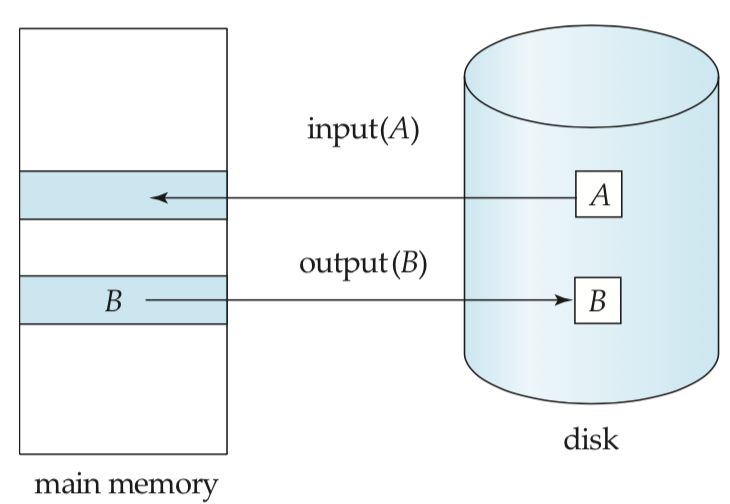
\includegraphics[width=0.5\textwidth]{images/block-storage}
\end{center}


\end{frame}


\begin{frame}
\frametitle{Manage Our Own}

In addition to this, the database has a small directory of what items are in the buffers (which resembles a page table in operating systems, actually). 

If some item is needed for a read or write, the directory is checked to find out if what we need is already in cache. 

If it is not then it must be retrieved from disk to be used. 

It might also be necessary to flush some of the data out to disk if there is no more space and we must replace a block.

\end{frame}

\begin{frame}
\frametitle{Pinned Blocks}

That sort of ``normal'' writing out to disk has some restrictions. 

Previous discussions of caching have covered the various algorithms and keeping track of whether the block was modified. 

There exists an additional restriction. 

This is whether or not the block is \alert{pinned} -- that is, forced to remain in memory and not permitted to be written to disk. 

This is often implemented as just a single bit in the block.
\end{frame}

\begin{frame}
\frametitle{Why Pinned?}

A very common example of why a page might be pinned by the recovery system is because it has been updated by a transaction that has not been committed.

If we wait for the transaction to commit, the block in question won't be written out to disk in a partially-updated state.

\end{frame}

\begin{frame}
\frametitle{Writing It Out}

Writing a block to the output via the \texttt{output} command itself might not result in immediately writing a particular block to disk. 

That block still might be needed for other operations. 

That can cause a bit of a headache because a crash before the output operation takes places means the data is lost... 

The recovery system can choose, however, to insist a block be written to disk immediately. 

That is called a \alert{force output} if a write command is explicitly issued.

\end{frame}

\begin{frame}
\frametitle{Ensuring Atomicity}

What we really want to avoid is that a transaction is incompletely recorded in the non-volatile storage, violating the atomicity of the transaction. 

The example we'll use is the standard banking sort of example. 

We want to transfer \$50 from account $A$ (initial balance, \$1000) to account $B$ (initial balance, \$2000). 

If the system crashed during the execution, after the write of the block containing $A$ has taken place but before the write of the block containing $B$ has? 

Volatile memory is lost in the crash so we don't know the fate of the transaction.

\end{frame}

\begin{frame}
\frametitle{After the Crash}

Under these circumstances, looking at the data usually does not tell us enough. 

If $A$ shows a balance of \$950 and $B$ a balance of \$2000, we know (from the setup of the example) that this is incorrect. 

The database system, however can't tell if those values are correct or incorrect without some additional information (just as we can't either). 

And as we have already discussed, we can solve this by writing the information to the log before performing the actual write.

\end{frame}

\begin{frame}
\frametitle{Writing the Log}
More formally, the log is a tuple of 4 elements: 

$T_{i}$, the transaction in question; 

$X_{j}$, the data element to be modified; 

$V_{1}$ the old value; and 

$V_{2}$ the new value. 

Other log records would indicate when a transaction begins, when it commits, or when it aborts. 

\end{frame}

\begin{frame}
\frametitle{Deleting the Log Data}

To prevent the log size from getting out of hand, we will need to eventually delete some old history. 

We could take the NTFS-like approach and delete transactions from the log once they are well and truly finished. 

But that, as we will soon see, is not actually what we do. 

\end{frame}

\begin{frame}
\frametitle{Do It Again}

These give us enough information to perform the undo or redo operations as described above. 

In the case of the bank transfer example, we can see that the step to change the balance of $A$ from \$1000 to \$950 has succeeded. 

The step to change the balance of $B$ from \$2000 to \$2050 has not. 

There are two valid paths for proceeding: undo the change to $A$ OR redo the change to $B$. 

Both produce consistent results.


\end{frame}


\begin{frame}
\frametitle{Undo or Redo?}

You might imagine that it is always preferable to redo the operation, but that can really only happen if the transaction has already committed... 

Otherwise we don't know what else the transaction was going to do.


\end{frame}


\begin{frame}
\frametitle{Multiple Undo/Redo}
As you might imagine, if there are multiple things to be undone or redone, the order matters to produce the correct result. 

If you don't believe that order matters, next time you bake a cake, first bake all the ingredients, then mix them. 

The redo approach then, requires us to scan the log from top to bottom, performing appropriate redo actions where necessary on each log record. 

This is efficient and sensible, preserving order and reading the log only once, sequentially.

\end{frame}

\begin{frame}
\frametitle{Let's... Undo Things}

The undo operation works a little differently. 

It restores data items to their old values, but also writes a log noting what it has done. 

The log records created are noted as ``redo-only'' because they don't contain the old (now-erased) value of the log record.

That looks like it's very strange, but we'll see shortly why this is so.

\end{frame}



\begin{frame}
\frametitle{Let's... Undo Things}

And when all undo operations for a given transaction are completed, an abort log record is put into the log to show that the undo is finished. 

This guarantees that every transaction will have either a commit or abort record in the log, even those that were unfinished at the time of the crash.

\end{frame}


\begin{frame}
\frametitle{Undo or Redo?}

With these rules in mind, given a log, how do we determine what transactions need to be undone or redone? 

Obviously, if a transaction does not have either a commit or abort log message it was unfinished and will be aborted. 

If a transaction has a commit in the log, it needs to be redone. But if a transaction has an abort in the log it needs to be redone as well.

\end{frame}

\begin{frame}
\frametitle{Undo or Redo?}
Wait, what? 

When a transaction is undone, we need to undo the changes with those redo-only log entries to make sure everything is put back where it should be.

\end{frame}


\begin{frame}
\frametitle{Transaction Log}

\begin{center}
	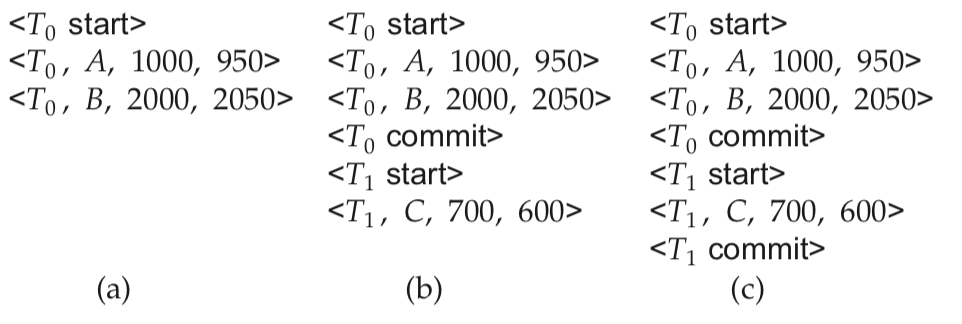
\includegraphics[width=0.7\textwidth]{images/transaction-log}
\end{center}

Let's see what happens if there's a crash at (a), (b), and (c).

\end{frame}

\begin{frame}
\frametitle{Undo or Redo?}

Remember that if a transaction aborts, the transaction is ``redone''. 

Redo-only statements are carried out to cancel out anything that was done before it. 

So the transaction might write a value to $X$ only to have it reversed by the subsequent operation before the abort.

\end{frame}


\begin{frame}
\frametitle{Forgetting History}

As just mentioned, the log structure we have means we write a lot into the log but never take anything out. 

And in theory to recover from a crash we have to scan the entire log and redo or undo anything needing to be redone or undone. 

This can be, however, a very long list. Repeating the redo operations many times does no harm, but it is a huge waste of time.

\end{frame}

\begin{frame}
\frametitle{Forgetting History}
What we'd like is to remove from the log any transactions that are well and truly done and we're sure a redo operation is totally redundant. 

We can remove them one at a time as the very last step of actually recording a transaction as done. 

That can require a lot of searching the log to find which one is the right one to remove. 

Instead, we can try to do this en masse through \alert{checkpoints}.


\end{frame}


\begin{frame}
\frametitle{Checkpoint}

A checkpoint is a particular place in the log where we ``save our progress''. 

If there is a crash we need only resume from the last checkpoint rather than starting at the beginning of the log. 

You are very likely already familiar with checkpoints, because they have been something you encountered in another context. 

Suppose everyone's favourite Italian plumber plunges to an untimely death... 

You can resume from some partial progress, such as the beginning of the level, or even some halfway point within the level.

You don't need to start the quest to save the princess from the very beginning.


\end{frame}

\begin{frame}
\frametitle{Performing a Checkpoint}

The steps to perform a checkpoint are:

\begin{enumerate}
	\item Write all logs currently in volatile storage to stable storage.
	\item Write all all modified buffer block to stable storage.
	\item Place a checkpoint record in the log.
\end{enumerate}

Transactions are not allowed to make changes to buffers or logs during the time a checkpoint is being created.

\end{frame}

\begin{frame}
\frametitle{Checkpoints}

The checkpoint record notes that it is a checkpoint and has a list $L$ of all transactions that are active at the time of the checkpoint. 

The checkpoint means that any transaction before that point in the log is completed and for sure put out to stable storage.

Those transactions do not need to be repeated. Excellent.

\end{frame}

\begin{frame}
\frametitle{Checkpoints}

If a crash occurs, we just look for the last checkpoint in the log. 

Then the only redo and undo operations that need to be performed are those on the transactions in the list $L$ and any that started after the checkpoint.

From there the routine works as we have previously described: 

For each transaction, redo or undo depending on the state of the transaction.
\end{frame}

\begin{frame}
\frametitle{Ancient History}

The checkpoint also allows us to get rid of some records once they become sufficiently old. 

Anything that is before the first transaction in $L$ of a checkpoint is ``ancient history'' and can be removed from the log.

\end{frame}

\begin{frame}
\frametitle{The Recovery Algorithm}

Recovery takes place in two phases, first the redo phase and then the undo phase (really). 

We start at the last checkpoint in the log and scan our way forward, then reverse direction and go back. 

\end{frame}


\begin{frame}
\frametitle{Redo Phase}

The \alert{redo phase} requires replaying updates of all transactions, scanning forward in the log from the last checkpoint. 

Even the ones that were rolled back (as we have seen) and including those transactions that were incomplete. 

We still do those operations, but we will note for later the incomplete transactions. 

\end{frame}

\begin{frame}
\frametitle{Redo Phase}

More formally:

\begin{enumerate}
	\item The list of transactions to be rolled back is set to the list $L$ of the last checkpoint record in the log.
	\item Each log operation is then carried out, both the ``regular'' and redo-only operations.
	\item If we encounter the start of a transaction marker for a new transaction, add that transaction to the list of transactions to be rolled back.
	\item If we reach an abort or commit statement for a transaction, remove that transaction from the list of transactions to be rolled back.
\end{enumerate}


\end{frame}

\begin{frame}
\frametitle{Undo Phase}

Following this phase of the process, we have identified all transactions that were incomplete (neither committed nor aborted) at the time of the crash. 

Then we have the \alert{undo phase}: 

Roll back all appropriate transactions in the list we have just generated in the redo phase. 

We scan the log backwards from the end moving up.

\end{frame}


\begin{frame}
\frametitle{Undo Phase}

\begin{enumerate}
	\item Whenever we find a record in the undo list, we perform the usual undo actions as if it was rollback of a failed transaction.
	\item When we reach the start log entry of a transaction we know we have undone all actions of that transaction, so we can put an abort record at the end of the log, and remove this transaction from the list.
	\item The undo phase terminates when the undo-list is empty (i.e., all incomplete transactions are properly undone).
\end{enumerate}

\end{frame}


\begin{frame}
\frametitle{Fixed?}


Following the undo phase, the database is in a consistent state again and new transactions can be permitted to begin... 

In other words, the system may begin normal operations.

The database is once again in a consistent state and all transactions have the atomic nature they promise. 

They have either completed successfully or it's as if they didn't happen at all.

Some operations were cancelled and potentially permanently lost, but the database is in a consistent state and that is the goal of the recovery process.

\end{frame}






\end{document}

